\documentclass[a4paper, 11pt]{article}
\usepackage{multirow}
\usepackage{soul}
\usepackage{graphicx}
\usepackage{amsmath}
\usepackage[export]{adjustbox}
\usepackage{float}
\usepackage[margin=1in]{geometry}
\usepackage{gensymb}
\usepackage{listings}
\usepackage{indentfirst}
\usepackage{xcolor}
% \usepackage[draft,nosingleletter]{impnattypo}

\usepackage{xcolor}

\definecolor{codegreen}{rgb}{0,0.6,0}
\definecolor{codegray}{rgb}{0.5,0.5,0.5}
\definecolor{codepurple}{rgb}{0.58,0,0.82}
\definecolor{backcolour}{rgb}{0.95,0.95,0.92}

\lstdefinestyle{mystyle}{
    backgroundcolor=\color{backcolour},   
    commentstyle=\color{codegreen},
    keywordstyle=\color{blue},
    numberstyle=\tiny\color{codegray},
    stringstyle=\color{codepurple},
    basicstyle=\ttfamily\footnotesize,
    breakatwhitespace=false,         
    breaklines=true,                 
    captionpos=b,                    
    keepspaces=true,                 
    numbers=left,                    
    numbersep=5pt,                  
    showspaces=false,                
    showstringspaces=false,
    showtabs=false,                  
    tabsize=2
}

\lstset{style=mystyle}

\begin{document}

\begin{center}
	\begin{tabular}{cc}
		\hline
		\multicolumn{2}{|c|}{\begin{tabular}[c]{@{}c@{}} \\ \LARGE \so{Informatyka w Medycynie - Laboratorium} \\ \\ \end{tabular}}         \\ \hline
		\multicolumn{2}{|c|}{\begin{tabular}[l]{@{}l@{}}\\\Large Wykrywanie naczyń dna siatkówki oka - projekt \\ \\ \end{tabular}}                      \\ \hline
		\multicolumn{1}{|l|}{\begin{tabular}[l]{@{}l@{}} \\ \hspace{2cm}Kierunek/semestr: Informatyka/6 \hspace{2cm} \\ \\ \end{tabular}} &
		\multicolumn{1}{|c|}{\begin{tabular}[l]{@{}l@{}} \\ Grupa: L16 \\ \\ \end{tabular}}                                                 \\ \hline
		\multicolumn{2}{|c|}{\begin{tabular}[c]{@{}c@{}}\\ Jakub Kwiatkowski 145356 \\Paweł Strzelczyk 145217  \\ \\ \end{tabular}}         \\ \hline
	\end{tabular}
\end{center}

\section{Opis projektu.}

Projekt został przygotowany w formie interaktywnego Jupyter Notebook.



Do przetwarzania obrazów oraz uczenia maszynowego wykorzystano język Python 3 oraz biblioteki:

\begin{itemize}
	\item numpy,
	\item matplotlib,
	\item skimage,
	\item OpenCV,
	\item pandas,
	\item ipython (ipywidgets, IPython),
	\item scikit-learn,
	\item joblib.
\end{itemize}


Do analizy przetwarzania obrazów oraz uczenia maszynowego skorzystano z bazy danych medycznych HRF (High-Resolution Fundus). Zawiera ona 45 zdjęć o wymiarach $3504\times2336$ px.
W projekcie wykorzystano 15 zdjęć dna oka zdrowych pacjentów. Do każdego zdjęcia jest dostępna ręczna segmentacja oraz maska pola widzenia.


\newpage

\section{Opis wykorzystanych metod wykrywania naczyń dna siatkówki oka.}
\subsection{Przetwarzanie obrazu.}
\paragraph{Algorytm przetwarzania.}
\subparagraph{Wczytanie obrazu.}
\begin{center}
	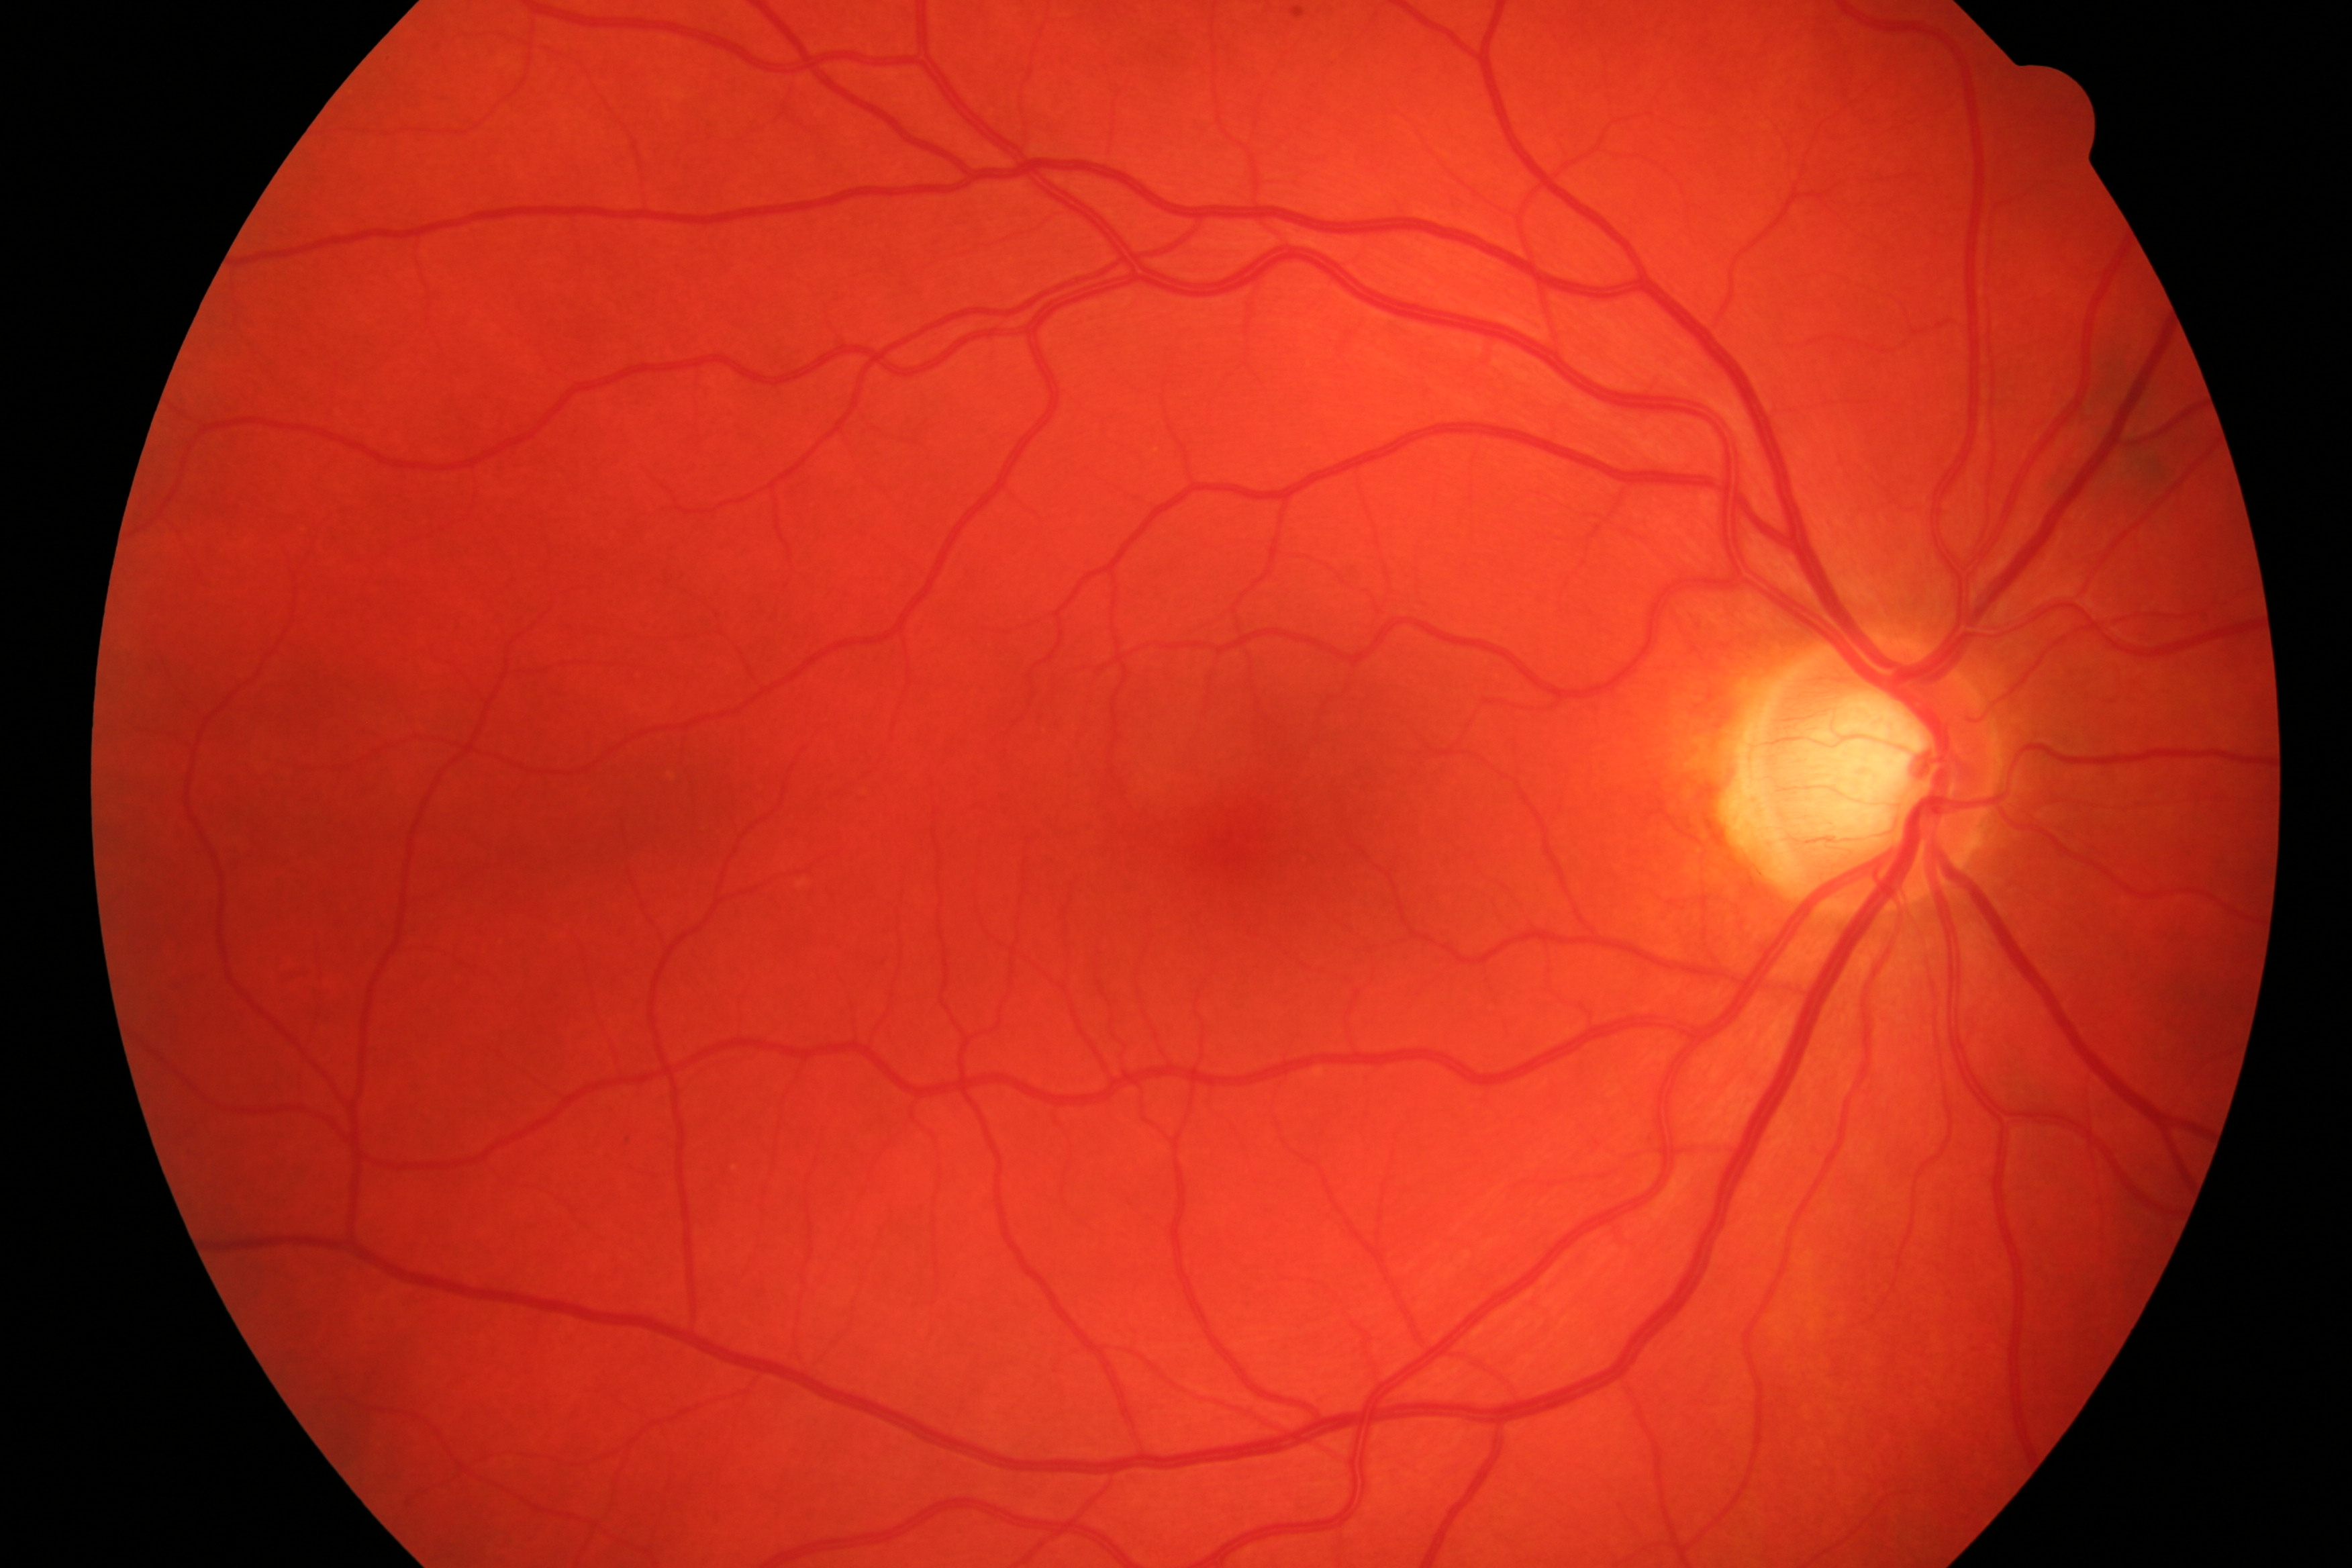
\includegraphics[width=0.8\textwidth]{./processing/input_image.png}
\end{center}

\subparagraph{Konwersja do przestrzeni barw CIELab.}


Konwersja w celu wyizolowania kanału l tejże przestrzeni, który dobrze odpowiada jasności obrazu.
\begin{center}
	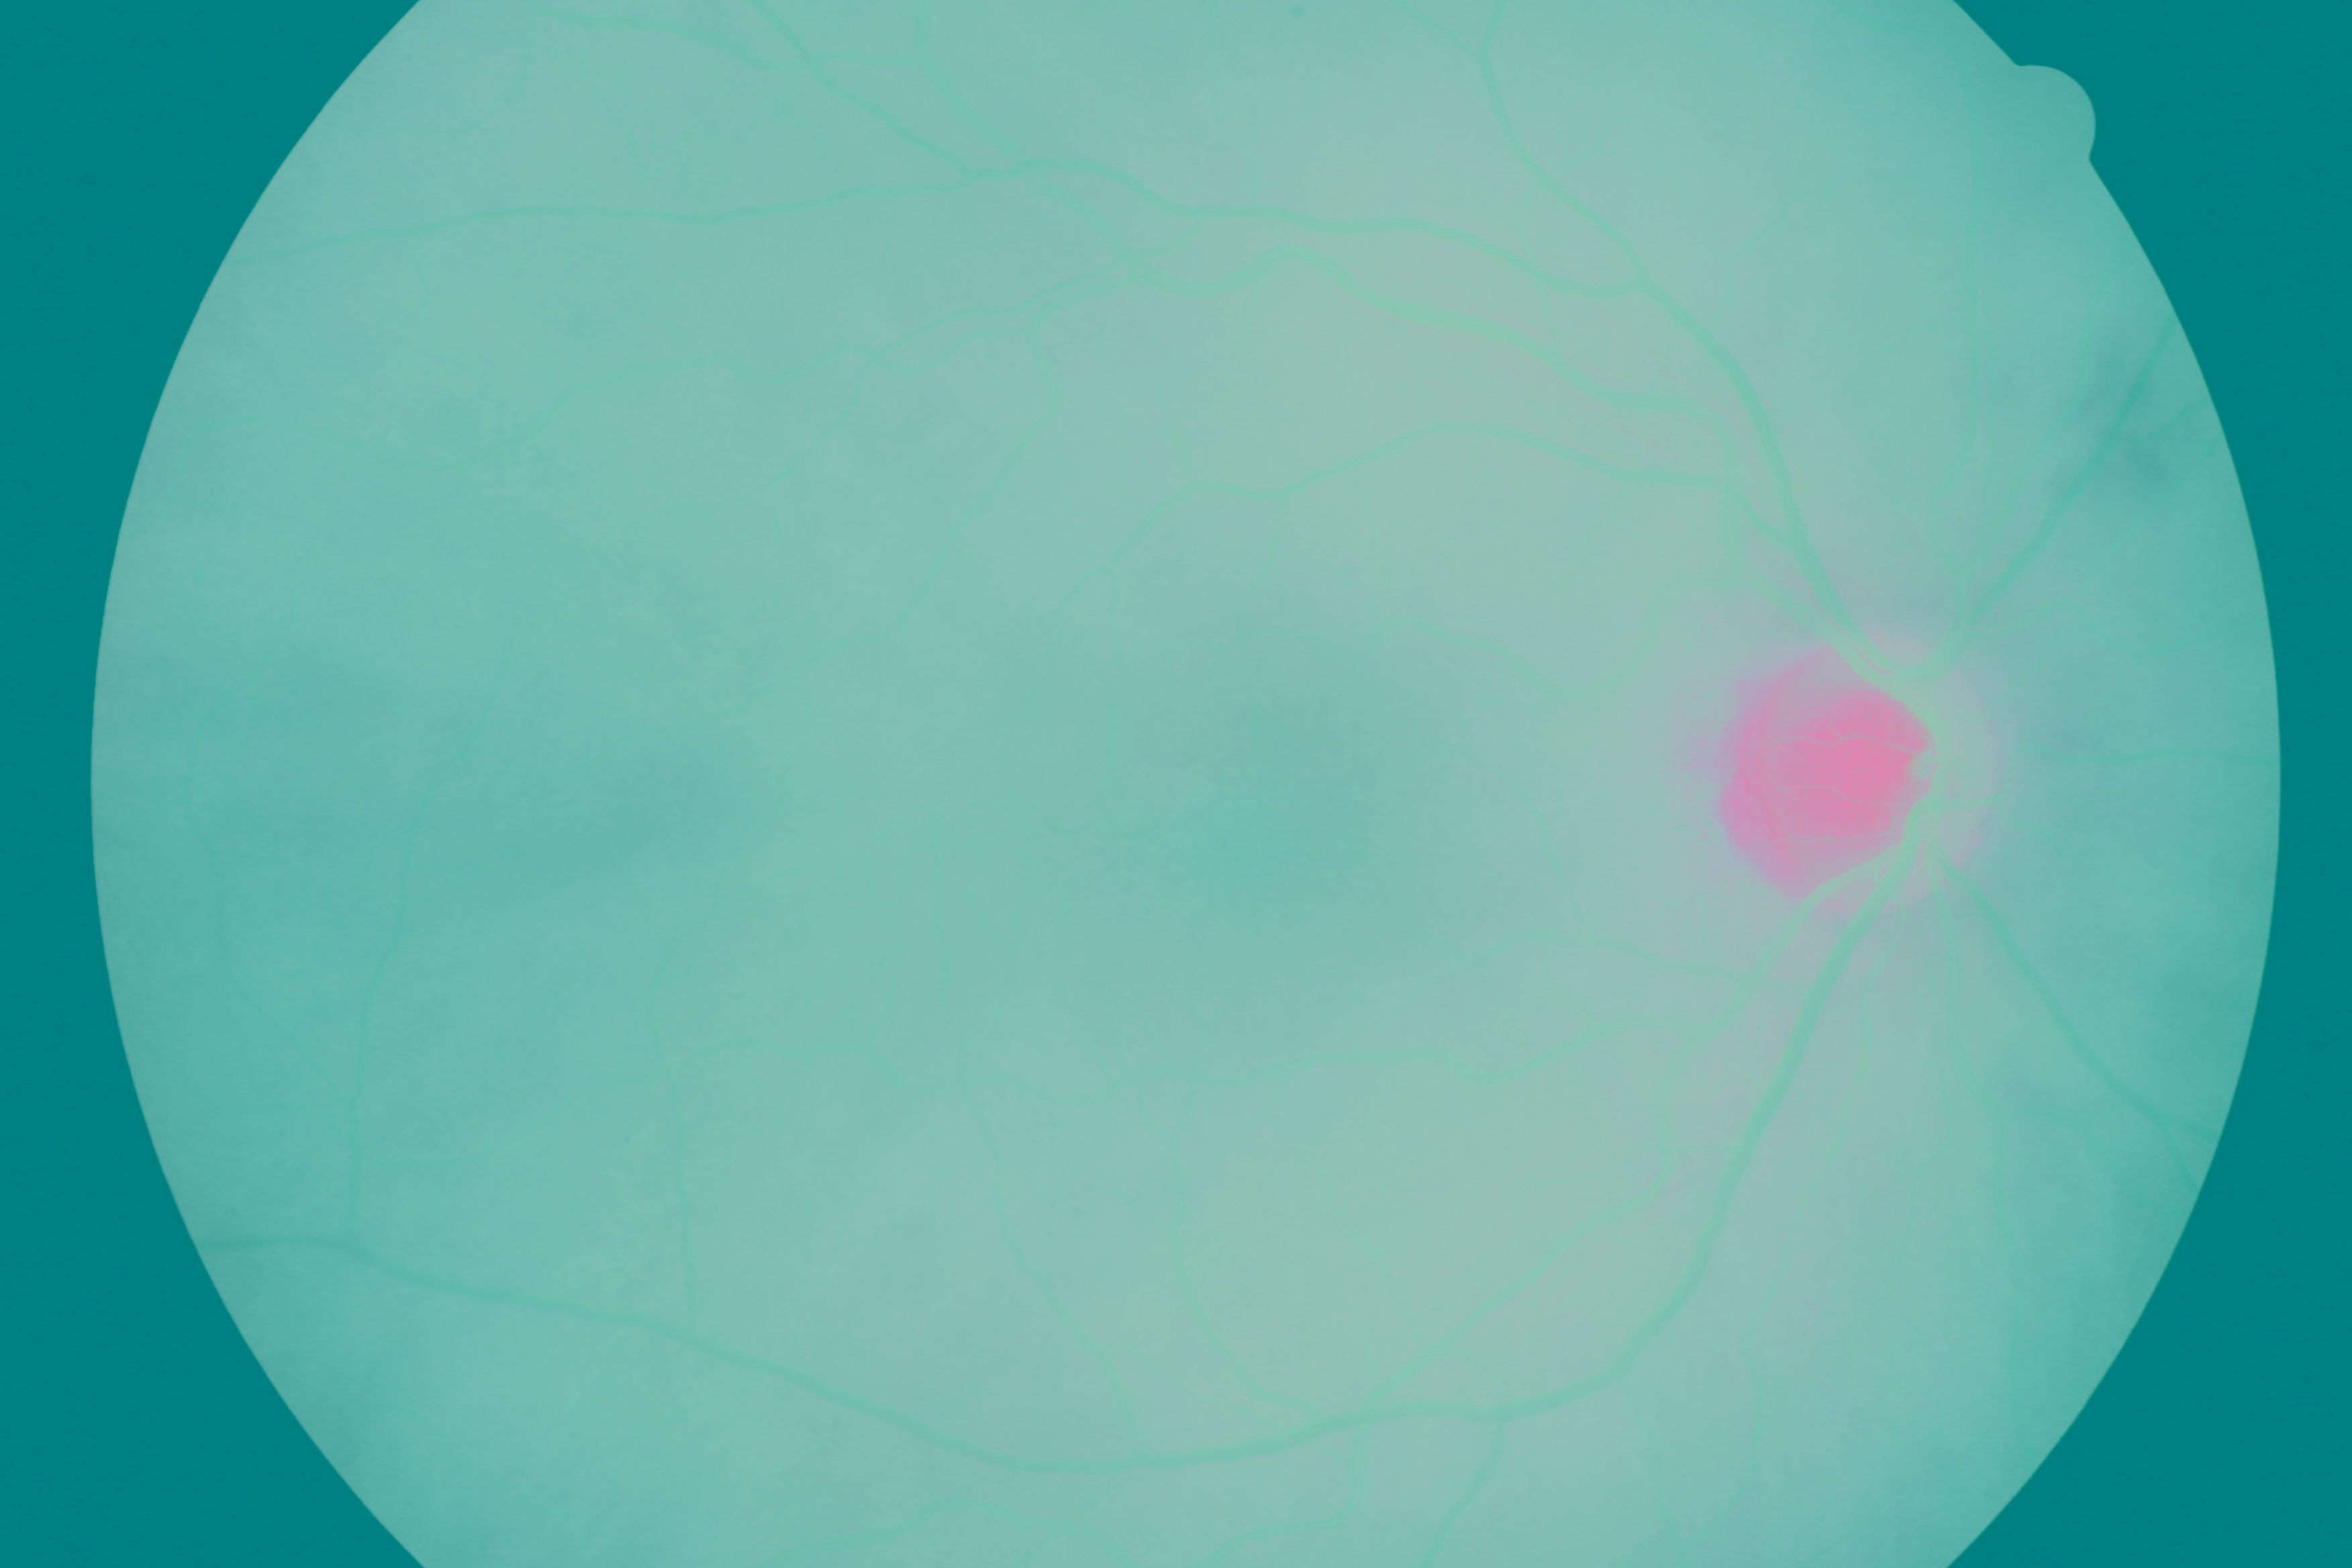
\includegraphics[width=0.8\textwidth]{./processing/lab_image.png}
\end{center}

\newpage
\subparagraph{Wyrównanie histogramu.}


Zastosowano wariant CLAHE wyrównania histogramu obrazu z progiem 3.
\begin{center}
	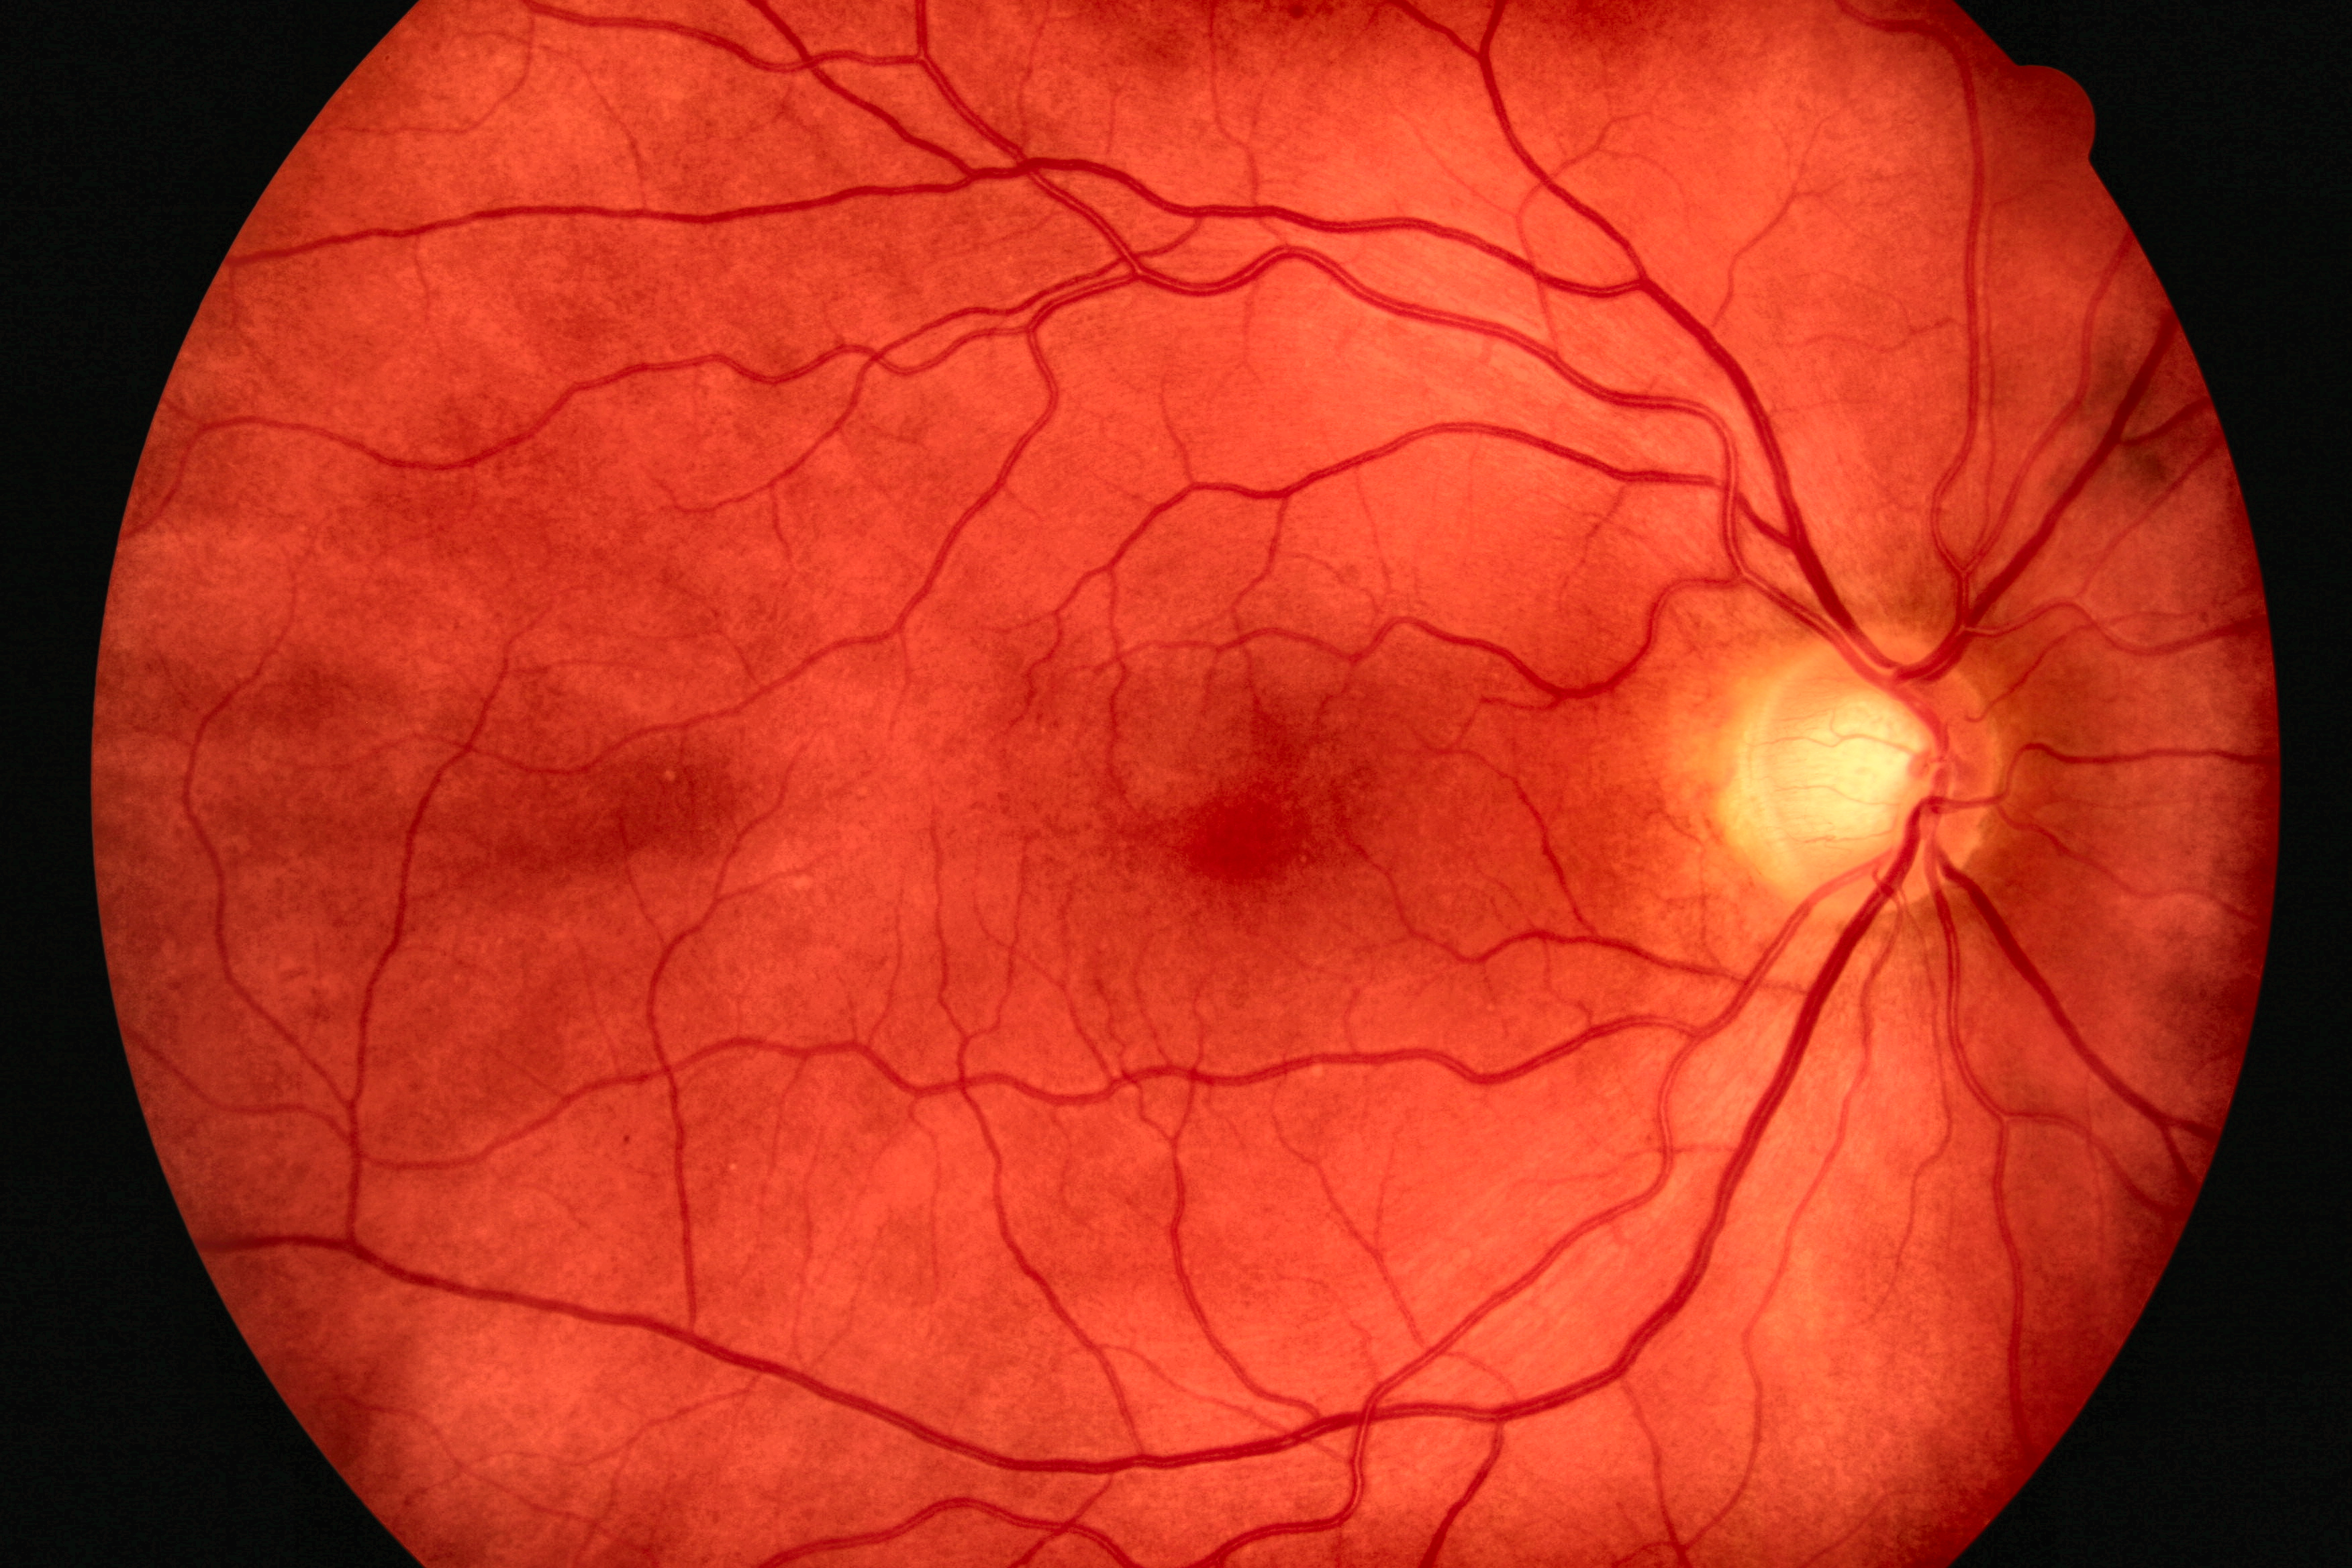
\includegraphics[width=0.8\textwidth]{./processing/clahe_image.png}
\end{center}
\subparagraph{Ekstrakcja kanału koloru zielonego.}


Naturalnie czerwone naczynia krwionośne są dobrze widoczne w zielonym kanale obrazu.
\begin{center}
	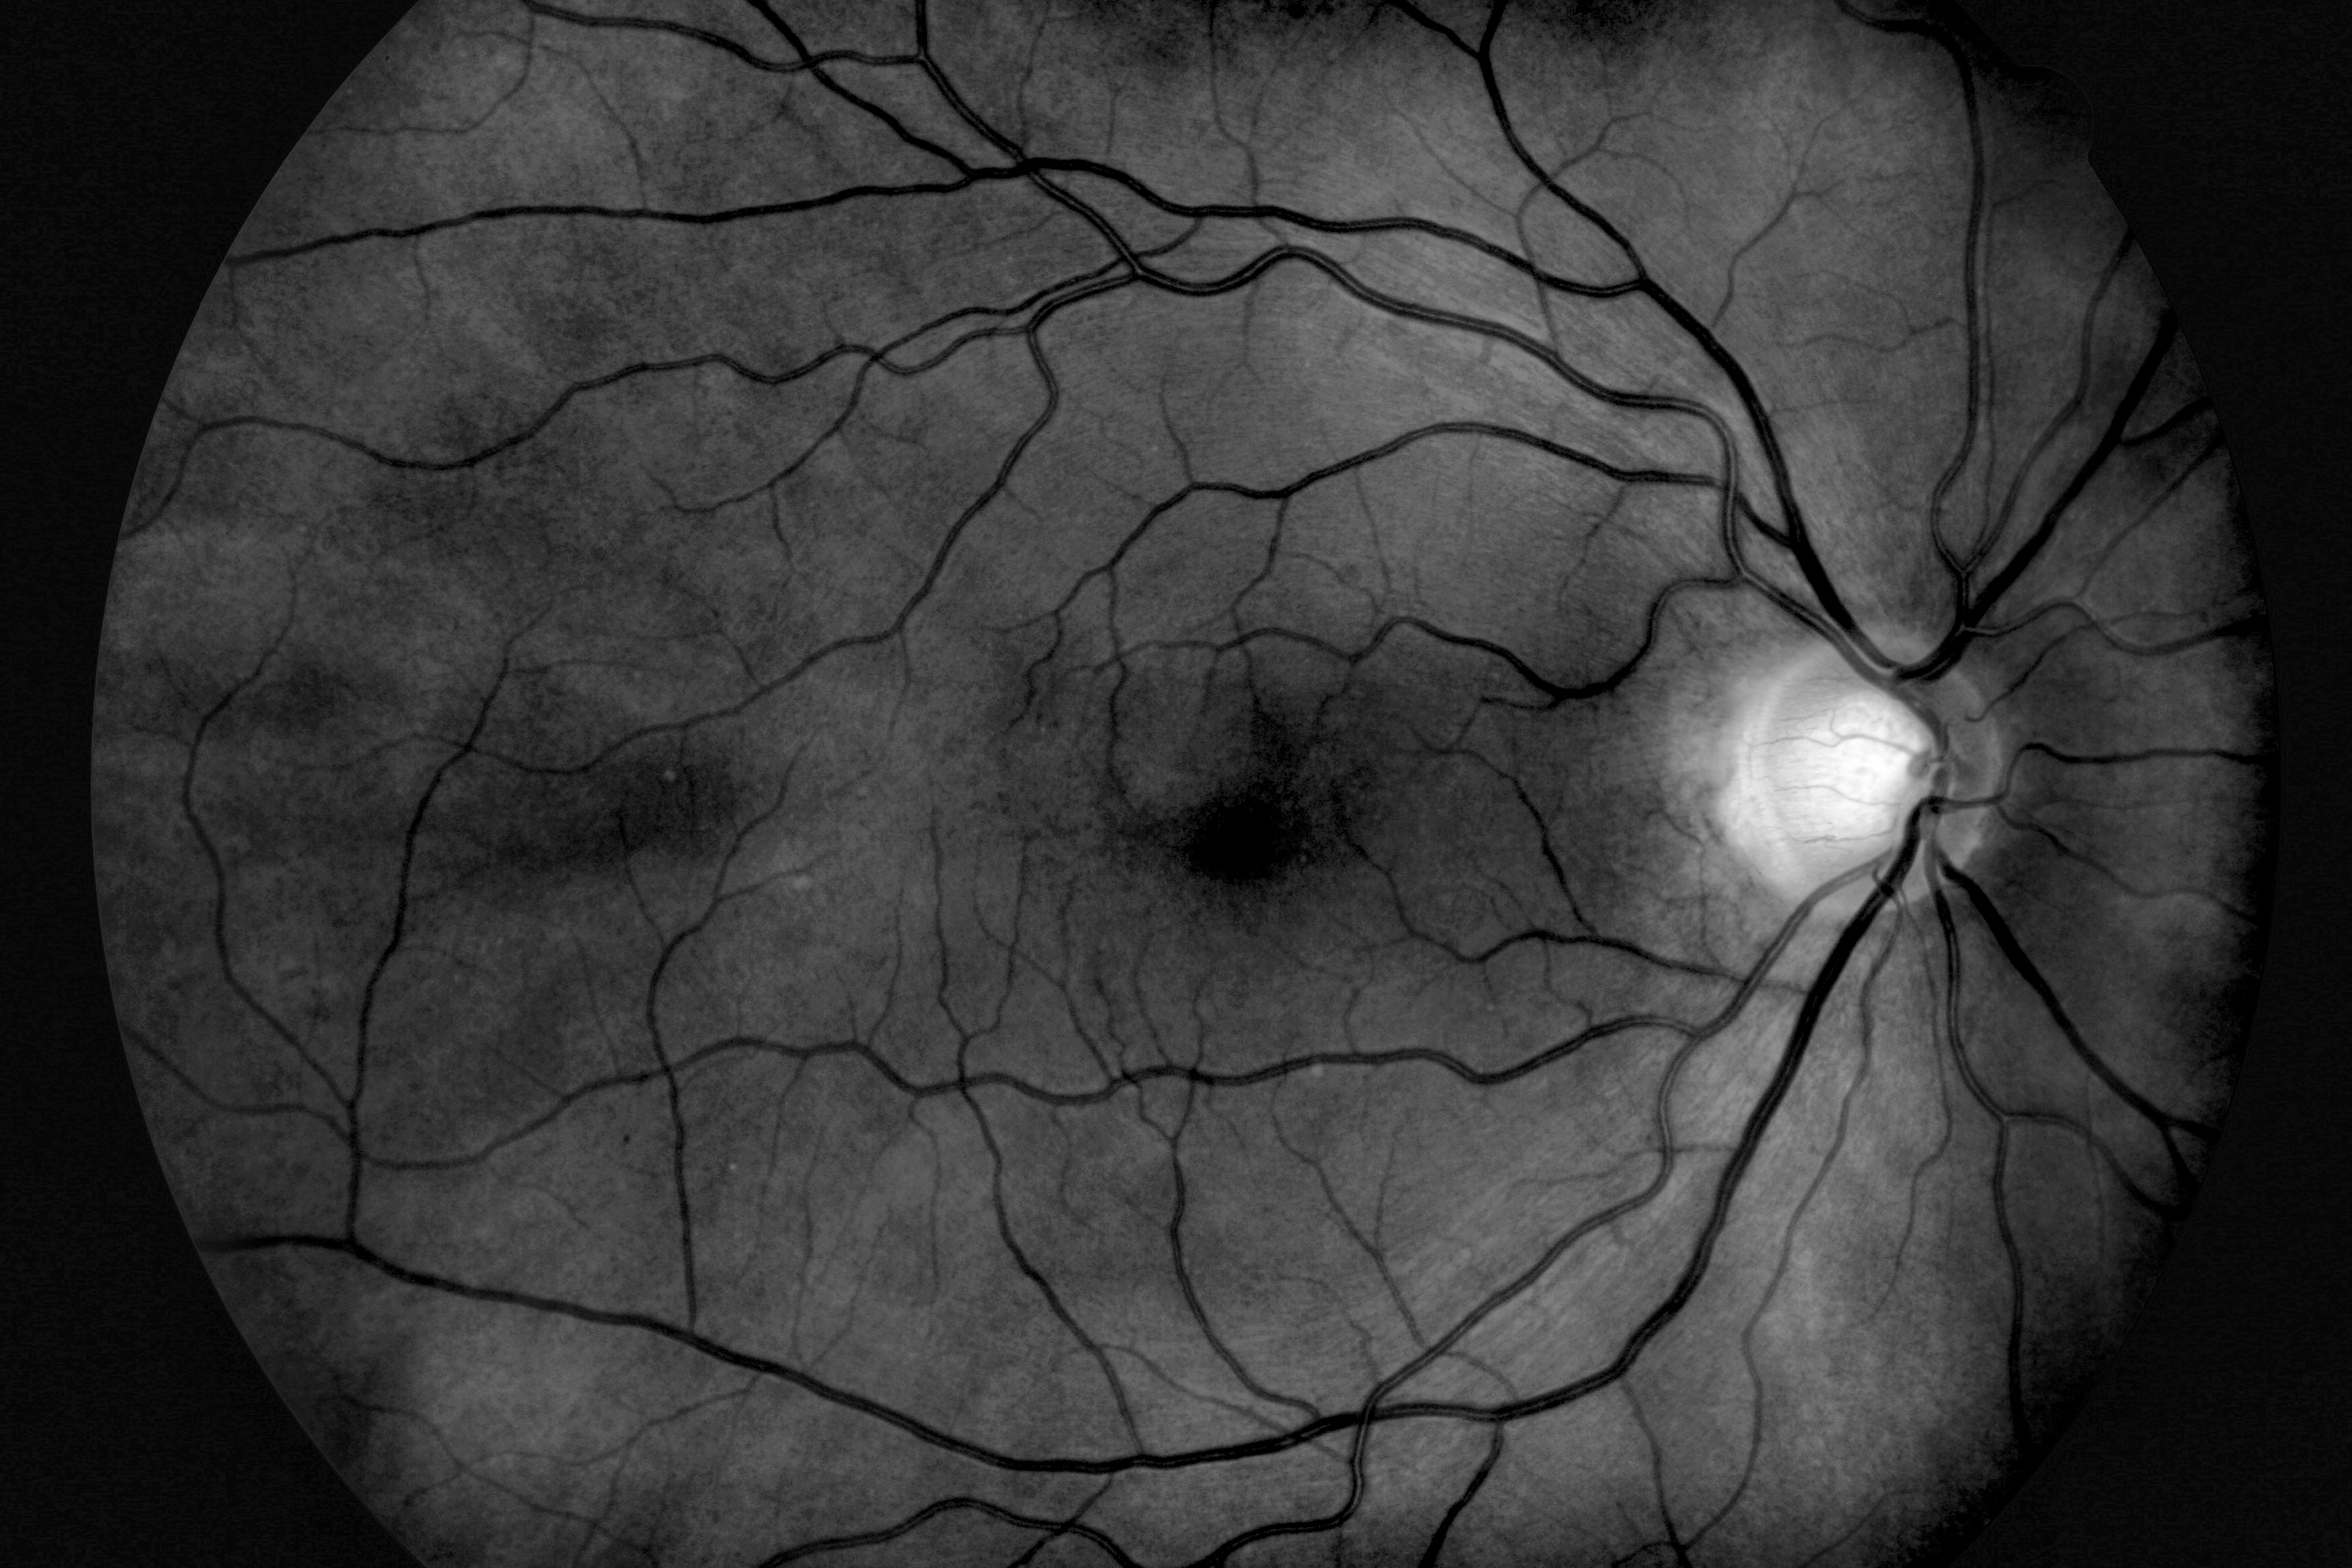
\includegraphics[width=0.8\textwidth]{./processing/green_image.png}
\end{center}

\newpage
\subparagraph{Filtr Frangi.}


Zastosowano filtr Frangi dostępny w bibliotece sckikit-image.
\begin{center}
	\includegraphics[width=0.8\textwidth]{./processing/frangi_image.png}
\end{center}
\subparagraph{Filtr progowy.}


Binarny przydział pikseli do klas - stwierdzenie czy dany piksel jest naczyniem. Jako próg odcięcia przyjęto średnią arytmetyczną wartość pikseli na obrazie, pomnożoną razy 0,45.
\begin{center}
	\includegraphics[width=0.8\textwidth]{./processing/thresh_image.png}
\end{center}

\newpage
\subparagraph{Przetwarzanie końcowe.}

Zastosowanie wbudowanych funkcji usuwania małych obiektów oraz dziur, następnie przeprowadzenie erozji oraz domknięcia morfologicznego.
\begin{center}
	\includegraphics[width=0.8\textwidth]{./processing/deblobed_image.png}
\end{center}
\paragraph{Uzasadnienie.}

Zdecydowano się na zastosowanie filtru Frangi'ego, ponieważ jest to dedykowana metoda wykrywania naczyń krwionośnych. Przetwarzanie wstępne miało na celu maksymalne zwiększenie kontrastu pomiędzy naczyniami a tłem. Przetwarzanie końcowe polegało na usunięciu niedoskonałości powstałych w wyniku przeprowadzenia filtrowania, m.in. na pozostawieniu jedynie ciągłych elementów o określonej powierzchni.

\paragraph{Miary statystyczne.}
\begin{center}
	\includegraphics[width=0.8\textwidth]{./processing/data.png}
\end{center}

\newpage


\subsection{Uczenie maszynowe - klasyfikator kNN.}
\paragraph{Podział obrazu na wycinki.}


Z uwagi na zasoby pamięciowe oraz dostępną moc obliczeniową, zdecydowano się na zmniejszenie wymiarów obrazów źródłowych do 20\% oryginalnej wielkości. Następnie dokonano podziału obrazu na wycinki o wymiarach $5\times5$, co jeden piksel (nakładające się). W tym celu skorzystano z funkcji dostępnej w bibliotece numpy - stride\_tricks.as\_strided().
\paragraph{Ekstrakcja cech.}

Do opisu wycinków skorzystano z:
\begin{itemize}
	\item średniej kolorów,
	\item wariancji kolorów,
	\item pierwszych siedmiu momentów Hu.
\end{itemize}
\paragraph{Metoda uczenia maszynowego.}

Jako metody uczenia maszynowego zdecydowano się na wykorzystanie klasyfikatora k najbliższych sąsiadów. Na podstawie jednego obrazu stworzono zbiór treningowy oraz testowy. Na ich podstawie nauczono oraz przetestowano model. Przyjęte parametry klasyfikatora to liczba sąsiadów $= 3$, liczba klas decyzyjnych$ = 2$, miara odległości - euklidesowa.

\paragraph{Ocena działania klasyfikatora na zbiorze hold-out.}

Wynik działania klasyfikatora - miary statystyczne zbioru hold-out testowego oraz przewidywanego.

\begin{itemize}
	\item trafność - 0,9609
	\item czułość - 0,8666
	\item specyficzność - 0,9777
	\item średnia G - 0,9204
\end{itemize}


\paragraph{Uzasadnienie.}

Wybór klasyfikatora kNN był pokierowany przede wszystkim poprawnie oznakowanym zbiorem danych, tzn. dla każdego piksela można stwierdzić, czy przynależy on do naczynia krwionośnego.
Ponadto, zbiór danych jest pozbawiony dużych odchyleń - takie parametry jak średnia kolorów lub wariancja, zawierają się w określonym przedziale w przypadku czarno-białego zdjęcia. Klasyfikator ten umożliwia także manipulowanie liczbą k, która ma znaczący wpływ na jakość klasyfikacji, dając możliwość znalezienia najlepszej jej wartości.

\newpage


\section{Wyniki.}
\subsection{Przetwarzanie obrazów.}
\begin{center}
	\includegraphics[width=\textwidth]{./processing/01_h.png}
	
	\includegraphics[width=\textwidth]{./processing/04_h.png}
	
	\includegraphics[width=\textwidth]{./processing/09_h.png}
	
	\includegraphics[width=\textwidth]{./processing/12_h.png}
	
	\includegraphics[width=\textwidth]{./processing/15_h.png}
	
\end{center}


\newpage
\subsection{Uczenie maszynowe.}

\begin{center}
	\includegraphics[width=\textwidth]{./ML/01_h.png}
	
	\includegraphics[width=\textwidth]{./ML/04_h.png}
	
	\includegraphics[width=\textwidth]{./ML/09_h.png}
	
	\includegraphics[width=\textwidth]{./ML/12_h.png}
	
	\includegraphics[width=\textwidth]{./ML/15_h.png}
	
\end{center}

\newpage

\section{Analiza porównawcza.}
\subsection{Przetwarzanie obrazów.}

\begin{center}
	
		\includegraphics[width=\textwidth]{./processing/data5.png}
		
\end{center}

\subsection{Uczenie maszynowe.}

\begin{center}
	
	\includegraphics[width=\textwidth]{./ML/data.png}
	
\end{center}

\subsection{Porównanie metod segmentacji.}

\paragraph{Obraz nr 1.}

\begin{center}
	
	\includegraphics[width=\textwidth]{./01_h.png}
	
\end{center}

\paragraph{Miary oceny przetwarzania.}
\begin{center}
	\includegraphics[width=\textwidth]{./processing/data1.png}
\end{center}

\paragraph{Miary oceny uczenia maszynowego.}
\begin{center}
	\includegraphics[width=\textwidth]{./ML/data1.png}
\end{center}

\newpage
\paragraph{Obraz nr 4.}

\begin{center}
	
	\includegraphics[width=\textwidth]{./04_h.png}
	
\end{center}

\paragraph{Miary oceny przetwarzania.}
\begin{center}
	\includegraphics[width=\textwidth]{./processing/data4.png}
\end{center}

\paragraph{Miary oceny uczenia maszynowego.}
\begin{center}
	\includegraphics[width=\textwidth]{./ML/data4.png}
\end{center}

\paragraph{Obraz nr 9.}

\begin{center}
	
	\includegraphics[width=\textwidth]{./09_h.png}
	
\end{center}

\paragraph{Miary oceny przetwarzania.}
\begin{center}
	\includegraphics[width=\textwidth]{./processing/data9.png}
\end{center}

\paragraph{Miary oceny uczenia maszynowego.}
\begin{center}
	\includegraphics[width=\textwidth]{./ML/data9.png}
\end{center}

\newpage
\paragraph{Obraz nr 12.}

\begin{center}
	
	\includegraphics[width=\textwidth]{./12_h.png}
	
\end{center}


\paragraph{Miary oceny przetwarzania.}
\begin{center}
	\includegraphics[width=\textwidth]{./processing/data12.png}
\end{center}

\paragraph{Miary oceny uczenia maszynowego.}
\begin{center}
	\includegraphics[width=\textwidth]{./ML/data12.png}
\end{center}

\paragraph{Obraz nr 15.}

\begin{center}
	
	\includegraphics[width=\textwidth]{./15_h.png}
	
\end{center}

\paragraph{Miary oceny przetwarzania.}
\begin{center}
	\includegraphics[width=\textwidth]{./processing/data15.png}
\end{center}

\paragraph{Miary oceny uczenia maszynowego.}
\begin{center}
	\includegraphics[width=\textwidth]{./ML/data15.png}
\end{center}








\end{document}